%%%%%%%%%%%%%%%%%%%%%%%%%%%%%%%%%%%%%%%%%%%%%%%%%%%%%%
% Thanks to Xu Minghao's work                        %
% I modify it into uchicago version                  %
% to not make new bug, I don't alter "Ritsumeikan"   %
% keywords in file. Pls feel free to use             %
%%%%%%%%%%%%%%%%%%%%%%%%%%%%%%%%%%%%%%%%%%%%%%%%%%%%%%

%%%%%%%%%%%%%%%%%%%%%%%%%%%%%%%%%%%%%%%%%%%%%%%%%%%%%%
% A Beamer template for Ritsumeikan University       %
% Author: Ming-Hao Xu (Xu Minghao)                   %
% Date:   April 2022.                                %
% LPPL Licensed.                                     %
%%%%%%%%%%%%%%%%%%%%%%%%%%%%%%%%%%%%%%%%%%%%%%%%%%%%%%

% \documentclass[aspectratio=64]{beamer}
\documentclass{beamer}
\usepackage{hyperref}
\usepackage[T1]{fontenc}
\usepackage{svg}
\usepackage{tikz}
\usepackage{graphicx}
\usepackage{wrapfig}

% other packages
\usepackage{latexsym,amsmath,xcolor,multicol,booktabs,calligra}
\usepackage{graphicx,pstricks,listings,stackengine}
\usepackage{algorithm2e}

\DeclareMathOperator*{\argmin}{argmin}


\author{Francis Moran \hspace{15pt} Ali Zafari}
\title{Proximal Algorithms for Basis Pursuit Denoising}
\subtitle{}
\institute{
    Electrical \& Computer Engineering Department\\
    Rutgers University
}
\date{\tiny Convex Optimization, Spring 2024}
\usepackage{presentation}

% defs
\def\cmd#1{\texttt{\color{green}\footnotesize $\backslash$#1}}
\def\env#1{\texttt{\color{blue}\footnotesize #1}}
\definecolor{deepblue}{rgb}{0,0,0.5}
\definecolor{deepred}{RGB}{153,0,0}
\definecolor{deepgreen}{rgb}{0,0.5,0}
\definecolor{halfgray}{gray}{0.55}

% listing settings
\lstset{
    basicstyle=\ttfamily\small,
    keywordstyle=\bfseries\color{deepblue},
    emphstyle=\ttfamily\color{deepred},    % Custom highlighting style
    stringstyle=\color{deepgreen},
    numbers=left,
    numberstyle=\small\color{halfgray},
    rulesepcolor=\color{red!20!green!20!blue!20},
    frame=shadowbox,
}

\begin{document}

\begin{frame}[plain, noframenumbering]
    \titlepage
    \vspace*{-0.6cm}
    \begin{figure}[htpb]
        \begin{center}
            % 
\includegraphics[keepaspectratio, scale=0.1]{figs/rutgers_seal_bw.jpg}
            \includesvg[height=0.38\textheight,keepaspectratio]{figs/rutgers_seal_color.svg}
        \end{center}
    \end{figure}
\end{frame}


\begin{frame}{}
    \begin{center}
        better late than never.\\
        \vspace{30pt}
        \pause
        Proves Wrong!
    \end{center}
    
\end{frame}

\begin{frame}{Papers of This Project}
    \begin{enumerate}
        \item N. Parikh, S. Boyd et al., “{\color{rutgerscarlet}Proximal Algorithms},” Foundations and Trends® in Optimization, 2014
        \vspace{10pt}
        \item (\textit{FISTA}) A. Beck and M. Teboulle, “{\color{rutgerscarlet}A Fast Iterative Shrinkage-Thresholding Algorithm for Linear Inverse Problems},” SIAM Journal on Imaging Sciences, 2009
        \vspace{10pt}
        \item (\textit{SpaRSA}) S. J. Wright, R. D. Nowak, and M. A. Figueiredo, “{\color{rutgerscarlet} Sparse Reconstruction by Separable Approximation},” IEEE Transactions on Signal Processing, 2009
    \end{enumerate}
\end{frame}


\begin{frame}    
\tableofcontents[sectionstyle=show,
subsectionstyle=show/shaded/hide,
subsubsectionstyle=show/shaded/hide]
\end{frame}



\section{Introduction \& Motivation}


\subsection{Unconstrained Optimization - Quick Recap}
\begin{frame}{Unconstrained Optimization - Quick Recap}
\begin{align*}
    \min_{x\in\mathbb{R}^n}f(x)
\end{align*}
\pause
\begin{itemize}
    \item If $f$ is convex and differentiable, $x^\star$ is a global minimizer if and only if $\nabla f(x^\star)=0$.
    \pause
    \item If $f$ is convex, any local minimzer is also a global minimizer.
    \pause
    \item If $f$ is strictly convex and has a global minimizer, then it is unique.
    \pause
    \item If $f$ is strongly convex then it has a global unique minimizer.
\end{itemize}
\end{frame}

\begin{frame}{Gradient Descent Method}
    \begin{algorithm}[H]
        
    	\textbf{given} a starting point $x_0\in\mathrm{dom} f$;\\
    	\Repeat{stopping criterion is satisfied}
     	{
      		$\Delta x_k=-\nabla f(x_k)$;\\
                \textit{Line Search}. Choose step size $\alpha_k$;\\
                \textit{Update}. $x_{k+1}:=x_{k}+\alpha_k\Delta x_k$;
      	}
    \end{algorithm}
    \pause\vspace{20pt}
    \begin{itemize}
        \item Differentiablity of $f$ is assumed.
        \pause
        \item Despite slower convergence rate than Newton's method, its simplicity of implementation makes it more desirable.
    \end{itemize}
\end{frame}

\begin{frame}{Convergence Rate of Gradient Descent}
    \begin{theorem}[GD Convergence]
         Let $f$ be a convex $L$-smooth function. Suppose that step size $\alpha_k=\frac{1}{L}$ is fixed for all iterations $k$. Gradient descent optimization yields
         \begin{align*}
            f_k(x)-f(x^\star)\leq\frac{L}{2 k}\|x_0-x^\star\|_2^2
         \end{align*}
         where $x^\star$ is any minizer of $f$.
    \end{theorem} 
    \pause
    \begin{itemize}
        \item In class we saw better rate with additional strong convexity assumption of $f$.
    \end{itemize}
\end{frame}


\subsection{Non-smooth Minimization}

\begin{frame}{Subgradient Method}
\begin{itemize}
    \item The subgradient method is the non-smooth version of gradient descent. The basic algorithm is straightforward, consisting of the iterations:
    \begin{align*}
        x_{k+1}=x_k-\alpha_k\Delta x_k
    \end{align*}
    where the $\Delta x_k$ is any member of $\partial f(x_k)$.
\end{itemize}
\pause\vspace{5pt}
\begin{definition}[Subgradient]
    Subgradient of function $f$ at $x$ is a vector $g\in\mathbb{R}^n$ such that
    \begin{align*}
        f(y)\geq f(x)+g^T(x-y) \;\;\forall y\in\mathrm{dom}f
    \end{align*}
    Collection of subradients at $x$ is called the subdifferential at $x$ denoting as $\partial f(x)$.
\end{definition}
\end{frame}

\begin{frame}{Convergence Rate of Subgradient Method}
    \begin{theorem}[Subgradient Non-convergence!]
    Let $f$ be a convex Lipschitz continuous function with $M>0$. Suppose that step size $\alpha_k=\alpha > 0$ is fixed for all $k$. Then
    \begin{align*}
        f_k^{\text{best}}-f(x^\star)\leq\frac{1}{2\alpha k}\|x_0-x^\star\|_2^2+\frac{\alpha M^2}{2}
    \end{align*}
    \end{theorem}
    \pause\vspace{10pt}
    \begin{itemize}
        \item Subgradient method does not guarantee a decrease at each iteration, so we keep the best after $k^{th}$ iteration, $f_k^{\text{best}}$.
        \pause
        \item For fixed step size, convergence is not guaranteed.
    \end{itemize}
\end{frame}

\begin{frame}{Convergence Rate of Subgradient Method - Cont'd}
    \begin{theorem}[Subgradient Convergence]
    Let $f$ be a convex Lipschitz continuous function with $M>0$. Suppose that step sizes satisfy $\alpha_k\rightarrow 0$ as $k\rightarrow\infty$ and $\sum_{k=1}^\infty\alpha_k=\infty$. Then the achievable rate for a general $f$ is
    \begin{align*}
        f_k^{\text{best}}-f(x^\star)\leq\frac{1}{\sqrt{k}}\|x_0-x^\star\|_2^2+Const.\frac{ M^2\log k}{\sqrt{k}}
    \end{align*}
    \end{theorem}
    \begin{itemize}
        \item This convergence rate is slow compared to gradient descent.
        \item The choice of step size heavily affects the convergence rate of subgradient method.
    \end{itemize}
\end{frame}

\subsection{Accelerating Algorithms}
\begin{frame}{Nestrov's Momentum Based Acceleration}
Using the same gradient descent method but with new updates:
\begin{eqnarray*}
\begin{aligned}
    &y_k = x_k+ \beta_k(x_k-x_{k-1})\\
    &x_{k+1}=y_k-\alpha_k\nabla f(y_k)
    \end{aligned}
\end{eqnarray*}
where $\beta_k=\frac{k-1}{k+2}$.
\pause
\begin{theorem}[Nestrov's Optimal Method]
Let $f$ be a convex $L$-smooth function ($L>0$). Nestrov's updates for suitable choices of step size $\alpha_k$ using gradient-based descent optimization yields:
    \begin{align*}
        f(x_k)-f(x^\star)\leq\frac{2L}{(k+1)^2}\|x_0-x^\star\|_2^2
    \end{align*}
\end{theorem}
\end{frame}

\section{Proximal Algorithms}

\subsection{Proximal Map Definition}
\begin{frame}{Proximal Map Definition}
\begin{definition}[Proximal Map]
    The proximal operator $\mathbf{prox}_{\alpha f}:\mathbb{R}^n\rightarrow\mathbb{R}^n$ of function $\lambda f:\mathbb{R}^n\rightarrow \mathbb{R}$ where $\alpha>0$:
    \begin{align*}
        \mathbf{prox}_{\alpha f}(x)=\argmin_{y}\left(f(y)+\frac{1}{2\alpha}\|y-x\|_2^2\right)
    \end{align*}
\end{definition}
\pause
\begin{itemize}
    \item The mapping itself includes an optimization problem.
    \pause
    \item Based on choice of $f$, the proximal mapping might have a closed form solution.
    \pause
    \item $f$ need not be differentiable.
\end{itemize}
\end{frame}

\begin{frame}{Gradient Descent Steps - Quadratic Upperbounds}
\textit{Recall}: For $L$-smooth convex function $f$ we can see that gradient descent step minimizes its quadratic upperbound at each iteration:
\begin{eqnarray*}
    \begin{aligned}
    f(x^\star)\leq f(y)&\leq f_{qup,x_k}(y)\qquad\forall y\in\mathrm{dom}f\\
    \pause
    &={\color{blue}f(x_k)+\nabla f(x_k)^T(y-x_k)+\frac{L}{2}\|y-x_k\|_2^2}\\
    \pause
    &=f(x_k)-\frac{1}{2L} \|\nabla f(x_k)\|_2^2 +\frac{L}{2}\|y-x_k+\frac{1}{L}\nabla f(x_k)\|_2^2
    \end{aligned}
\end{eqnarray*}
$y=x_k-\frac{1}{L}\nabla f(x_k)$ minimizes the last term.\\
\pause\vspace{20pt}
Proximal map showed itself:
\begin{align*}
\color{blue}x_{k+1}=\mathbf{prox}_{\frac{1}{L} f_{lin,x_k}}(x_k)=x_k-\frac{1}{L}\nabla f(x_k)
\end{align*}
\end{frame}

\subsection{Proximal Gradient Descent}
\begin{frame}{Proximal Gradient Descent}
Consider $f(x)=g(x)+h(x)$ where $g$ is $L$-smooth and convex and $h$ is convex.\\
\vspace{10pt}
\pause
Let's only consider proximal map for linear approximate of $g$, as we did for gradient descent update:
\begin{eqnarray*}
    \begin{aligned}
    x_{k+1}&=\mathbf{prox}_{\alpha_k f_{g_{lin,x_k}}}(x_k)\\
    \pause
    &=\argmin_{x}\left(g(x_k)+\nabla g(x_k)^T(x-x_k)+\frac{1}{2\alpha_k}\|x-x_k\|_2^2+h(x)\right)\\
    \pause
    &=\argmin_{x}\left(-\frac{\alpha_k}{2} \|\nabla g(x_k)\|_2^2 +\frac{1}{2\alpha_k}\|x-x_k+\alpha_k\nabla g(x_k)\|_2^2+h(x)\right)\\
    \pause
    &=\argmin_{x}\left(\frac{1}{2\alpha_k}\|x-x_k+\alpha_k\nabla g(x_k)\|_2^2+h(x)\right)\\
    \pause
    &=\mathbf{prox}_{\alpha_kh}(x_k-\alpha_k\nabla g(x_k))
    \end{aligned}
\end{eqnarray*}
\end{frame}

\subsection{Convergence Analysis}
\begin{frame}{Proximal Method Convergence Analysis}
    \begin{theorem}[Proximal Convergence]
        Consider $f(x)=g(x)+h(x)$ where $g$ is $L$-smooth and convex and $h$ is convex. Using fixed step size $\alpha_k=\frac{1}{L}$, and denoting $x^\star$ as the minimizer of $f$:
        \begin{align*}
            f(x_k)-f(x^\star)\leq\frac{L}{2k}\|x_0-x^\star\|_2^2
        \end{align*}
    \end{theorem}
    \pause
    \begin{itemize}
        \item Shining result is that the non-smooth optimization has similar behavior like gradient descent for smooth function. (Much faster than subgradient method!)
        \pause
        \item Easy computation of $\mathbf{prox}_{h}$ is assumed.
    \end{itemize}
\end{frame}

\begin{frame}{Question to be Answered}
\begin{center}
Can we accelerate proximal gradient descent?
% \\
% \vspace{20pt}
% (perhaps the same way we did for gradient descent, using momentum)
\end{center}
\end{frame}


\section{Basis Pursuit DeNoising (BPDN)}

% \subsection{Problem Definition}

\begin{frame}{BPDN - Problem Definition}
\begin{align*}
    \min_{\mathbf{x}\in\mathbb{R}^n}\;\; \|\mathbf{y}-A\mathbf{x}\|_2^2+\lambda \|\mathbf{x}\|_1
\end{align*}
where $\mathbf{y}\in\mathbb{R}^m$ is the measurement signal, $\mathbf{x}\in \mathbb{R}^n$ is the signal of interest to be recovered from the measurement $\mathbf{y}$, the matrix $A\in\mathbb{R}^{m\times n}$ is a known sensing matrix (usually $m<n$) and $\lambda\geq0$.\\
\vspace{5pt}
\begin{itemize}
    \pause
    \item $g:=\|.\|_2$ is $L$-smooth and convex.
    \pause
    \item $h:=\lambda\|.\|_1$ is not differentiable but convex.
    \pause
    \item Proximal map of $h$ is easy to compute (soft thresholding):
    \begin{equation*}
        \mathbf{prox}_{h}(x)=\mathrm{sign}(x)\max\{|x|-\lambda, 0\}
    \end{equation*}
    \pause
    \item Minimizing this problem using proximal gradient descent is called {\color{rutgerscarlet}Iterative Shrinkage-Thresholding Algorithm} (ISTA) in the literature.
\end{itemize}
\end{frame}

% \subsection{Equivalent Problems}

% \begin{frame}{BPDN - Equivalent Problems}
% BPDN can be generalized to a wide range of problems:
% \begin{itemize}
%     \item 
% \end{itemize}
% \end{frame}

\section{Accelerated Proximal Methods}


\subsection{FISTA}

\begin{frame}{Fast ISTA - Core Idea}
\begin{itemize}
    % \item Can we do the same momentum speeding for the proximal algorithms as we did for gradient descent algorithms?
    \item The idea stems from momentum-based acceleration we saw for gradient descent method.
    \item Current estimates are updated based on history of two previous updates.
    \item Convergence rate has been derived analytically and shows its proven advantage over the regular proximal gradient descent method. 
\end{itemize}
\end{frame}



\begin{frame}{FISTA - Algorithm}
Consider $f(x)=g(x)+h(x)$ where $g$ is $L$-smooth and convex and $h$ is convex.\\
\vspace{20pt}
\begin{algorithm}[H]
        
    	\textbf{given} $y_1 = x_0 \in \mathbb{R}^n, t_1 =1$;\\
    	\Repeat{stopping criterion is satisfied}
     	{
      		$x_k = \mathbf{prox}_{\frac{1}{L}h}(y_k-\frac{1}{L}\nabla g(y_k))$;\\
                $t_{k+1} = \frac{1 + \sqrt{1 + 4t_k^2}}{2}$;\\
                $y_{k+1} = x_k + \frac{t_k - 1}{t_{k+1}} (x_k - x_{k-1})$;
      	}
    \end{algorithm}
\pause
\vspace{10pt}
\begin{itemize}
    % \item $p_L$ is the basic iterative shrinking method
    \item Main difference to ISTA is that the proximal operator is evaluated at a linear combination of two previous points instead of only the last one.
\end{itemize}

\end{frame}

\begin{frame}{FISTA - Convergence Analysis}
    \begin{theorem}[FISTA Convergence]
        Consider $f(x)=g(x)+h(x)$ where $g$ is $L$-smooth and convex and $h$ is convex. Using fixed step size $\alpha_k=\frac{1}{L}$, and denoting $x^\star$ as the minimizer of $f$:
        \begin{align*}
            f(x_k)-f(x^\star)\leq\frac{2L}{(k+1)^2}\|x_0-x^\star\|_2^2
        \end{align*}
    \end{theorem}
    \pause
    \begin{itemize}
        \item For regular proximal gradient (\textit{e.g.,} ISTA) we had:
        \begin{align*}
            f(x_k)-f(x^\star)\leq\frac{L}{2k}\|x_0-x^\star\|_2^2
        \end{align*}
    \end{itemize}
\end{frame}



\subsection{SpaRSA}

\begin{frame}{SpaRSA - Core Idea}
\begin{itemize}
    \item The ISTA algorithm is modified heuristically to speed up convergence.
    \item The step size $\alpha_k$ is chosen heuristically based on a Barzilai-Borwein Spectral Method.
    \item As SpaRSA tends to slow down extremely when $\lambda$ is small, a method, called "continuation" is used to avoid that, by warm-starting the from the solution of the problem for a larger value of $\lambda$.
\end{itemize}
\end{frame}

\begin{frame}{Barzilai-Borwein Spectral Method}
\begin{itemize}
    \item It is a gradient method with step sizes inspired by Newton's method but without involving the Hessian.
    \pause
    \item Barzilai-Borwein approach chooses $\alpha'_k$ where $\alpha'_kI_{n\times n}$ be closest to the Hessian of $f$ over the last step.
    \pause
    \item With $r_k := \nabla f (x_k) - \nabla f (x_{k-1})$ and $ s_k := x_k - x_{k-1}$, we find $\alpha'_k$ such that $\alpha'_k s_k \approx r_k$, \textit{i.e.,}
    \begin{align*}
        \alpha'_k = \underset{\alpha'}{\argmin} \| \alpha' s_k - r_k \|_2^2=\frac{s_k^Tr_k}{s_k^Ts_k}
    \end{align*}
    \vspace{20pt}
    \begin{center}
        (Notation: $\alpha'_k$ is playing the role of $\frac{1}{\alpha_k}$ in previous slides)
    \end{center}
\end{itemize}

\end{frame}

\begin{frame}{SpaRSA - Algorithm}
Consider $f(x)=g(x)+h(x)$ where $g$ is $L$-smooth and convex and $h$ is convex.\\
\vspace{20pt}
\begin{algorithm}[H]
\textbf{Given}

    \textbf{$\eta >1 ,[0 <\alpha'_{min} < \alpha'_{max}], x_0 \in \mathbb{R}^n$}

    \Repeat{stopping criterion is satisfied}    
    {
        $\alpha'_k \in [\alpha'_{min}, \alpha'_{max}]$; \hspace{10pt}(Safeguarded Barzilai-Borwein)

        \Repeat{$x_{k+1}$ satisfies an acceptance criterion}
            {$x_{k+1} = \mathbf{prox}_{\frac{1}{\alpha'_k}h}(x_k-\frac{1}{\alpha'_k}\nabla g(x_k))$;\\
            $\alpha'_{k+1} \xleftarrow{} \eta \alpha'_k$;
            }
        $k \xleftarrow{} k + 1$;
    }
\end{algorithm}
    
\end{frame}

\begin{frame}{SpaRSA - Cont'd}

    \begin{itemize}
        \item Acceptence Criterion of $x_{k+1}$
        \pause
        \begin{itemize}
            \item Naive solution: to accept any solution of the proximal mapping. No monotone convergence is guaranteed.
            \pause
            \item Accept if objective value is slightly smaller than the maximum of $M$ past iterations:
            \begin{align*}
                f(x_{k+1})\leq \max_{i\in \{\text{M-last iterations}\}} f(x_i)-\frac{\sigma}{2}\alpha'_k\|x_{k+1}-x_k\|_2^2
            \end{align*}
            where $\sigma\in(0,1)$.  Although again no monotone convergence is guaranteed, but in practice it performs well.
        \end{itemize}

        \pause
        \item Stopping Criterion of Algorithm
        \pause
        \begin{itemize}
            \item As simple as comparing the relative change in the objective function with a small fixed value $\mathrm{tol} > 0$:
            \begin{align*}
                \frac{|f(x_{k+1})-f(x_k)|}{f(x_k)}\leq \mathrm{tol}
            \end{align*}
        \end{itemize}
        
    \end{itemize}
\end{frame}

\section{Numerical Experiments}

\begin{frame}{Image Deblurring}
\begin{itemize}
    % \item BPDN problem for 'cameraman' image
    \item BPDN problem where signal of interest $x$ is the wavelet coefficients of the image.
    \item Image passed through Gaussian blur with variance of 3

    
\end{itemize}

\begin{figure}[H]
    \centering
    \begin{tikzpicture}
        % Image 1
        \node[anchor=south west,inner sep=0] (image1) at (0,0) {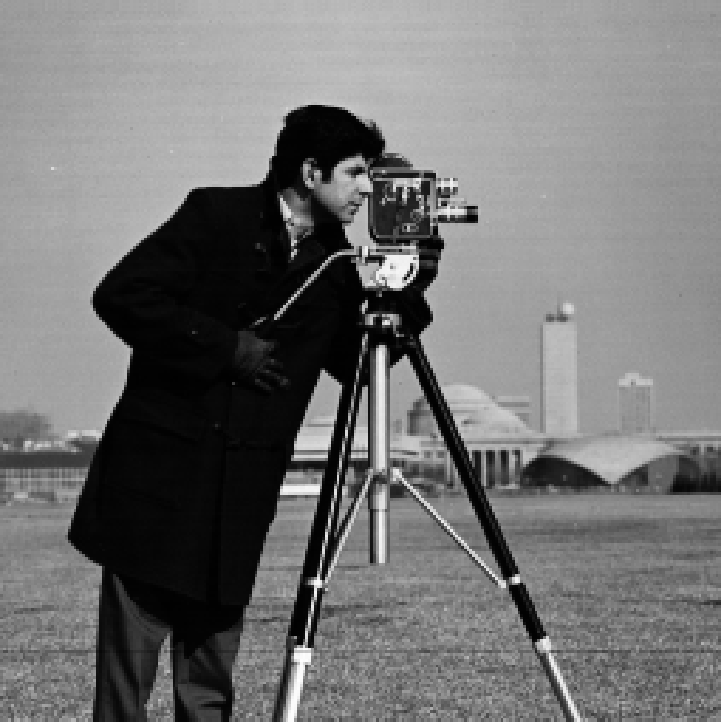
\includegraphics[width=0.4\textwidth]{figs/orig.png}};
        \node[above] at (image1.north) {Original};        
        % Image 2
        \node[anchor=south west,inner sep=0] (image2) at (0.55\textwidth,0) {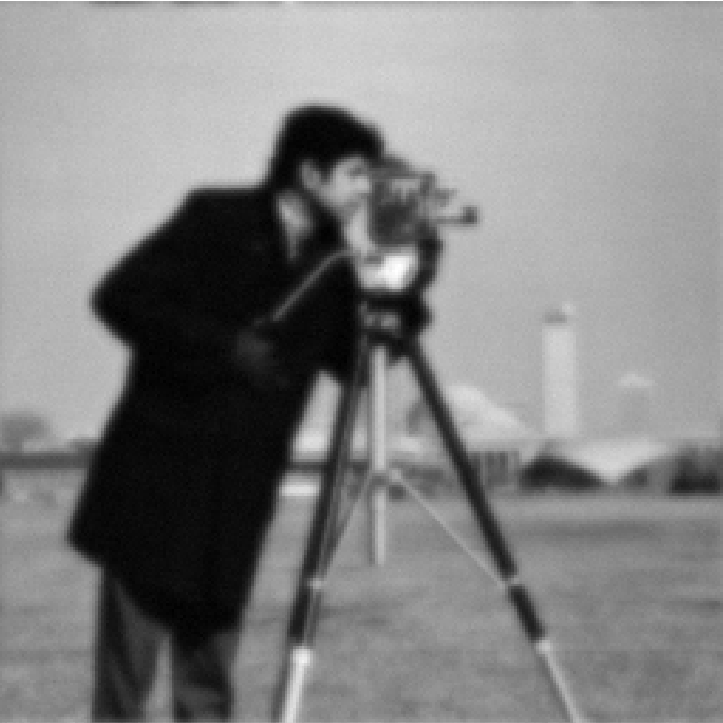
\includegraphics[width=0.4\textwidth]{figs/noisy.png}};
        \node[above] at (image2.north) {Blurred};
    \end{tikzpicture}
    \caption{Original and Blurred Cameraman Image.}
    \label{fig:camera-combined}
\end{figure}

\end{frame}




\begin{frame}{Image Deblurring}
% Recovered from all 3 algs
    \begin{figure}[H]
        \centering
        \begin{tikzpicture}
            % Image 1
            \node[anchor=south west,inner sep=0] (image1) at (0,0) {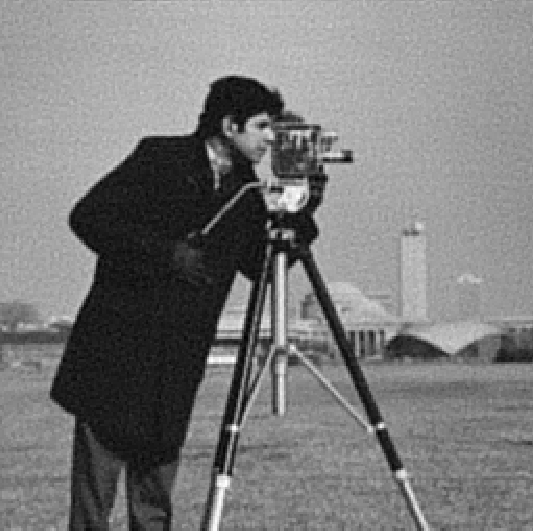
\includegraphics[width=0.3\textwidth]{figs/rec_ista.png}};
            \node[above] at (image1.north) {ISTA};        
            % Image 2
            \node[anchor=south west,inner sep=0] (image2) at (0.35\textwidth,0) {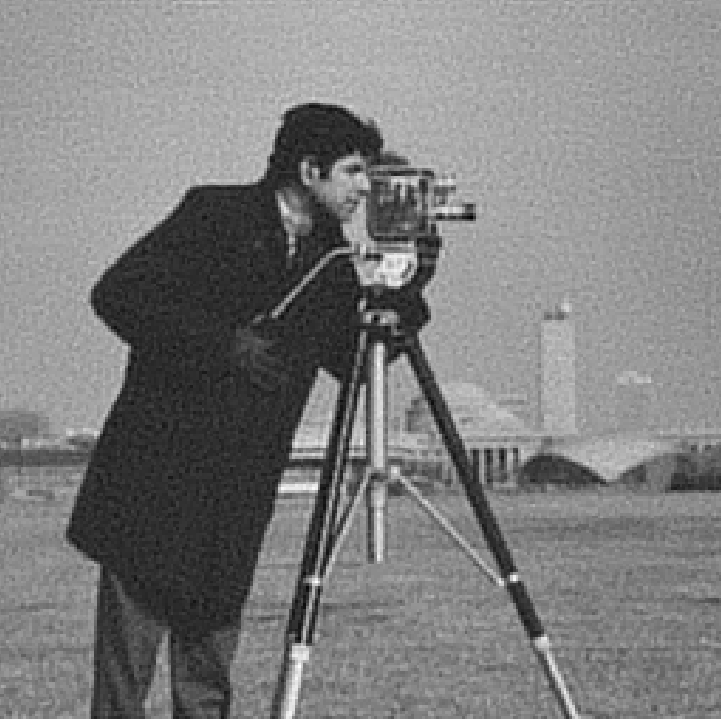
\includegraphics[width=0.3\textwidth]{figs/rec_fista.png}};
            \node[above] at (image2.north) {FISTA};        
            % Image 3
            \node[anchor=south west,inner sep=0] (image3) at (0.7\textwidth,0) {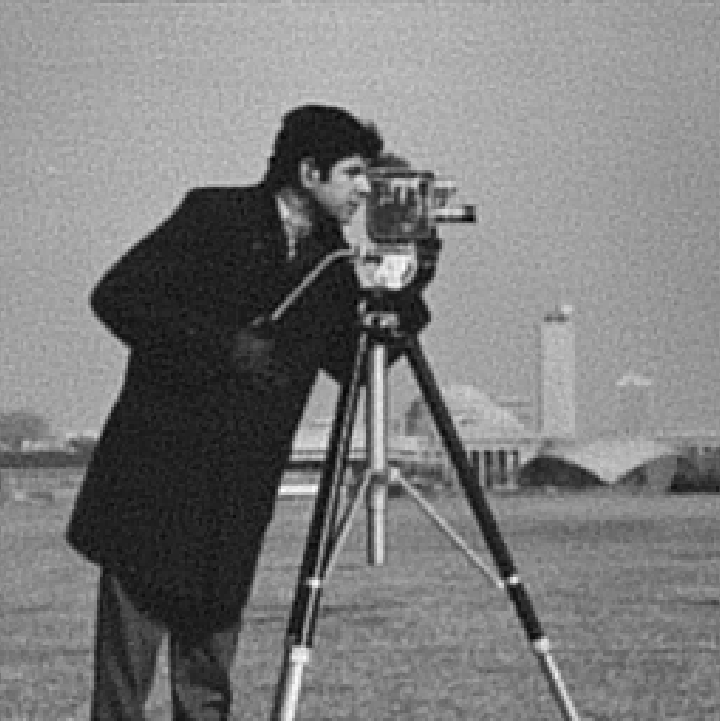
\includegraphics[width=0.3\textwidth]{figs/rec_sparsa.png}};
            \node[above] at (image3.north) {SpaRSA};
        \end{tikzpicture}
        \caption{Recovered Images from each Algorithm.}
        \label{fig:combined}
    \end{figure}
\end{frame}

\begin{frame}{Image Deblurring}
    \begin{figure}
        \centering
        \begin{tikzpicture}
            % Image
            \node[anchor=south west,inner sep=0] (image) at (0,0) {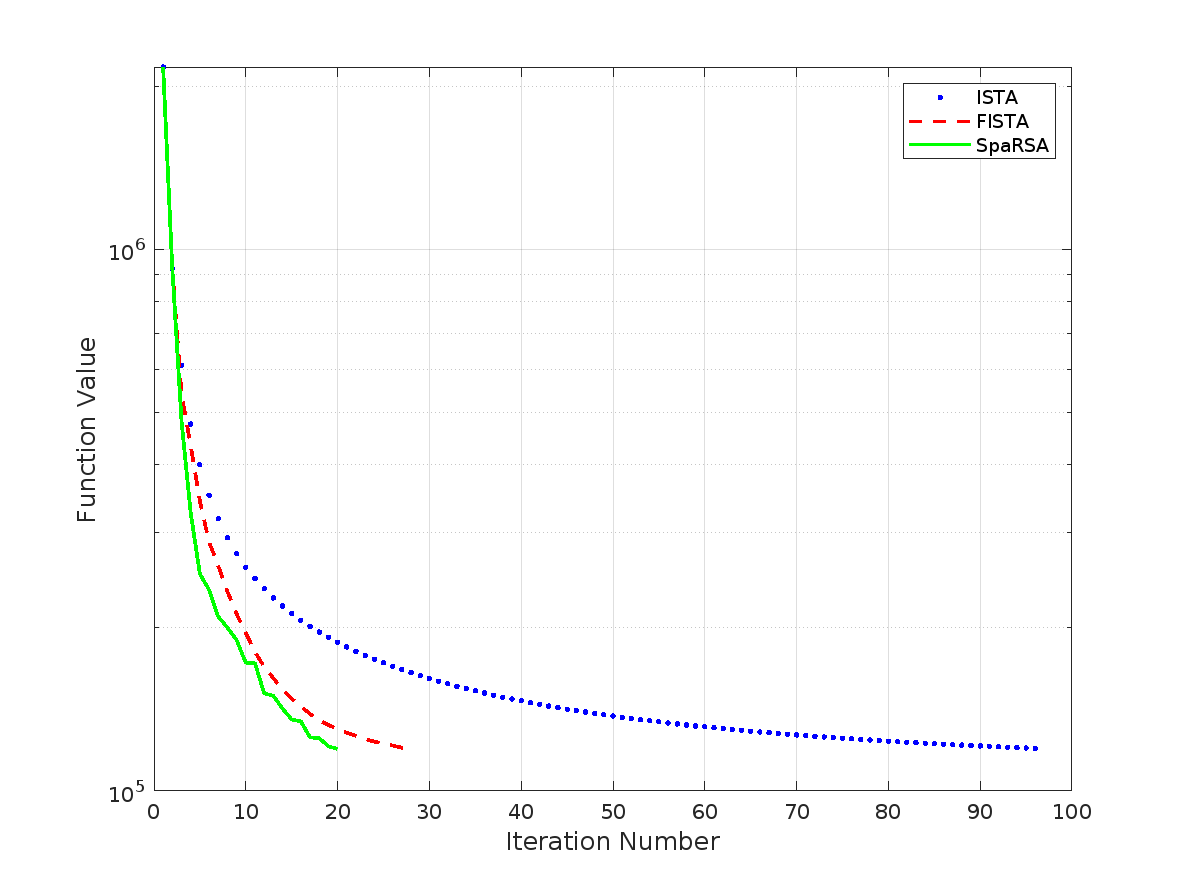
\includegraphics[width=0.8\textwidth]{figs/plot.png}
            };
        \end{tikzpicture}
        \caption{Objective Value vs Iteration Number of ISTA, FISTA, and SpaRSA}
        \label{fig:plot-combined}
    \end{figure}
\end{frame}

\section{Conclusions}
\begin{frame}{Conclusions \& Learning Outcomes}
    \begin{itemize}
        \item Exciting thing: the type of analysis we learned over the semester are so common over these very technical publications.
        \pause
        \item Proximal methods are like the gradient method for non-smooth objective functions, although with having in mind to have a simple proximal map.
        \pause
        \item Although FISTA provides a very well-established convergence analysis, SpaRSA presents better results in practice.
        \pause
        \item Both FISTA and SpaRSA are general accelerated proximal gradient descent methods, not limited to BPDN problem.
    \end{itemize}
\end{frame}


\section{References}

\begin{frame}[allowframebreaks]
    \bibliography{refs}
    
    \nocite{*} % used here because no citation happens in slides
    % if there are too many try use:
    \tiny\bibliographystyle{ieee}
    % \tiny\bibliographystyle{alpha}
\end{frame}

\end{document}